% !TEX program = pdflatex
% Kakutani-KMS theory of ligand-induced conformational phase transitions (integrating Papers I-VII)
\documentclass[11pt,reqno]{amsart}

\usepackage[T1]{fontenc}
\usepackage[utf8]{inputenc}
\usepackage{lmodern}
\usepackage[a4paper,margin=27mm]{geometry}
\usepackage{amsmath,amssymb,amsthm,mathtools}
\usepackage{booktabs}
\usepackage{graphicx}
\graphicspath{{./}{../figures/}}
\usepackage{array}
\usepackage{microtype}
\usepackage{enumitem}
\usepackage{xcolor}
\usepackage[colorlinks=true,linkcolor=blue!60!black,citecolor=blue!60!black,urlcolor=blue!60!black]{hyperref}

\theoremstyle{plain}
\newtheorem{theorem}{Theorem}[section]
\newtheorem{lemma}[theorem]{Lemma}
\newtheorem{proposition}[theorem]{Proposition}
\newtheorem{corollary}[theorem]{Corollary}
\theoremstyle{definition}
\newtheorem{definition}[theorem]{Definition}
\theoremstyle{remark}
\newtheorem{remark}[theorem]{Remark}
\numberwithin{equation}{section}

\newcommand{\dd}{\mathrm{d}}
\newcommand{\EE}{\mathbb{E}}
\newcommand{\PP}{\mathbb{P}}
\newcommand{\Z}{\mathbb{Z}}
\newcommand{\N}{\mathbb{N}}
\newcommand{\Rr}{\mathbb{R}}
\newcommand{\DKI}{\mathrm{DKI}}
\newcommand{\CKI}{\mathrm{CKI}}
\newcommand{\Xib}{\Xi_\beta^{\mathrm{drug}}(S)}
\newcommand{\Wtail}{W_{\mathrm{tail}}}
\newcommand{\gEM}{\gamma_{\mathrm{EM}}}
\newcommand{\DCKI}{\Delta\mathrm{CKI}}

\renewcommand{\abstractname}{Summary}
\setlength{\emergencystretch}{2em}

\title[Kakutani--KMS theory of ligand-induced conformational phase transitions]{Kakutani--KMS Theory of Ligand-Induced Conformational Phase Transitions:\\ Measure-Class Obstructions, Covariance Criticality, and Tail Allostery in Computational Pharmacology}

\author[Z. Chen]{Zhengyi Chen}
\address{Guangxi Key Laboratory of Drug Discovery and Optimization, School of Pharmacy, Guilin Medical University, Guilin 541199, P.~R. China}
\email{chenzhengyi@glmc.edu.cn}

\author[R. Chen]{Ruqing Chen}
\address{GUT Geoservice Inc., Montreal, Qu\'ebec, Canada}
\email{ruqing@hotmail.com}

\thanks{DOI: \href{https://doi.org/10.5281/zenodo.23042828}{10.5281/zenodo.23042828}.\newline Sources: \url{https://github.com/Ruqing1963/kakutani-statistical-pharmacology-synthesis}.\newline This article integrates the series \emph{Statistical Pharmacology via Kakutani Dichotomy}, Papers I--VII \cite{ChenChen2026I,ChenChen2026II,ChenChen2026III,ChenChen2026IV,ChenChen2026V,ChenChen2026VI,ChenChen2026VII}, whose sources, code and data are archived under the DOIs listed in the Data availability statement.}
\thanks{This project was supported by the National Natural Science Foundation of China (No.~22464010), the Guangxi Natural Science Foundation of China (No.~2025GXNSFAA069294), and the 2025 Bagui Youth Top Talent Project.}
\date{29 September 2026}

\subjclass[2020]{Primary 92C40, 60G15; Secondary 82B26, 46L30, 49Q22, 62H12}
\keywords{Kakutani dichotomy, Feldman--H\'ajek theorem, KMS states, Bhattacharyya distance, conformational ensembles, allostery, spontaneous symmetry breaking, Wasserstein distance, free-energy perturbation, molecular dynamics}

\begin{document}

\begin{abstract}
Two ligands can produce the same local structure in a binding pocket and the same binding free energy while driving the protein into different global conformational ensembles. We make this statement precise and quantitative. Conformational ensembles are treated as measures on infinite-dimensional configuration spaces, where Kakutani's and Feldman--H\'ajek's theorems leave only two possibilities: equivalence or mutual singularity. The \emph{blindness theorem} shows that every functional of the pocket marginal, and every functional of the single-residue marginals, is blind to this dichotomy. Identical pocket laws, identical per-residue fluctuations and identical binding free energies are compatible with mutually singular global ensembles. A companion proposition shows that a ligand acting only through a pocket-local energy cannot produce singularity, so global inequivalence requires the reorganisation of an extended coupling network. We then assemble the theory that measures such reorganisations:
\begin{itemize}[leftmargin=*]
\item the marginal drug Kakutani index DKI and its critical decay exponent $\alpha_c=\tfrac12$, with the universal doubling increment $A\ln2$;
\item the correlated index CKI, its exact decomposition into mean, commuting and rotation parts, and the $99.95\%$ dominance of the covariance term in correlated networks;
\item the spectral Feldman--H\'ajek criticality of collective modes, in amplitude ($\Delta\ln\lambda_i$) and in rotation ($\theta_i$);
\item the KMS temperature scaling $\beta_c=1$ and tail allostery, in which a pocket contribution of order $10^{-3}$ coexists with a distal contribution growing as $N^{1-1/\beta}$;
\item the chemical obstruction group $\Xib\cong(\Z/2\Z)^{A_\beta}$ that classifies broken conformational phases, with a relative-entropy staircase of one $\ln2$ per threshold;
\item the cone-geodesic Wasserstein cost $\Wtail$ of converting one broken phase into another, and the sampling advantage of cooperative alchemical paths;
\item an estimation pipeline for molecular-dynamics trajectories with shrinkage, null subtraction and shell scaling, together with a tail-augmented molecular representation $z_{\mathrm{local}}\oplus z_{\mathrm{symmetry}}\oplus z_{\mathrm{tail}}$.
\end{itemize}
Every constant quoted is taken from the reproducible computations of the series. All numerical evidence comes from analytic models and synthetic trajectories with known ground truth; validation on all-atom molecular dynamics of real protein--ligand systems remains to be done.
\end{abstract}

\maketitle
\tableofcontents

%%%%%%%%%%%%%%%%%%%%%%%%%%%%%%%%%%%%%%%%%%%%%%%%%%%%%%%%%%%%%%%%%%%%%%%%%%%%%%%
\section{Introduction: the blindness of local and tensorized invariants in drug discovery}
\label{sec:intro}

\subsection*{The problem}
Structure-based design ranks ligands by quantities that are \emph{local}: the fit of a pose in a pocket, a root-mean-square deviation of pocket atoms, a docking score, an alchemical estimate of the binding free energy $\Delta G_{\mathrm{bind}}$. It is widely recognised that function is a property of the whole conformational ensemble \cite{MWC1965,Motlagh2014}. Ligands that look alike in the pocket can differ in efficacy, in bias between signalling outcomes, or in their allosteric effect on a distal site \cite{Bowman2012,Motlagh2014}. What has been missing is a mathematical statement of \emph{how much} a local description can miss, and a theory that measures what it misses.

The mathematical setting we use is that of infinite product measures and Gaussian measures, where two classical theorems apply. Kakutani's theorem \cite{Kakutani1948} says that two infinite products of equivalent probability measures are either equivalent or mutually singular, according to whether the product of the Hellinger affinities of the factors is positive or zero. The Feldman--H\'ajek theorem \cite{Feldman1958,Hajek1958} gives the same dichotomy for Gaussian measures. The same dichotomy governs the phase transitions of the KMS states of Bost--Connes systems and their localized generalisations \cite{BostConnes1995,Chen2026}, where a transition is a \emph{tail event}: it is decided by the convergence of an infinite sum and is invisible to any finite factor. The series \emph{Statistical Pharmacology via Kakutani Dichotomy} \cite{ChenChen2026I,ChenChen2026II,ChenChen2026III,ChenChen2026IV,ChenChen2026V,ChenChen2026VI,ChenChen2026VII} transported this mechanism to conformational ensembles. This article integrates its results into one theory.

\subsection*{The blindness theorem}
Let the conformational state of a protein be a sequence $x=(x_i)_{i\ge1}$ of local coordinates (residue switches, dihedral states, collective modes), and let a ligand $L$ induce an ensemble $P_L$ on the space of such sequences. A \emph{pocket observable} is a functional $\Phi(P_L)$ that depends on $P_L$ only through its marginal on a finite set $F$ of pocket coordinates. Examples are the distribution of pocket geometries and hence any pocket RMSD, a docking score, and a binding free energy computed from an interaction energy $U_L(x_F)$ with the pocket. A \emph{tensorized observable} depends only on the single-coordinate marginals $(P_L)_i$, $i\ge1$. Examples are per-residue fluctuations (RMSF), per-residue occupancies, and the first-order index of Section~\ref{sec:dki}.

\begin{theorem}[Blindness of local and tensorized invariants]\label{thm:blind}
\begin{enumerate}[label=\textup{(\arabic*)},leftmargin=*]
\item \emph{Local blindness.} For every finite set $F$ there are product measures $P=\bigotimes_i\mathrm{Bern}(p_i)$ and $Q=\bigotimes_i\mathrm{Bern}(q_i)$ with $P|_F=Q|_F$ that are mutually singular. Every pocket observable takes the same value on $P$ and $Q$.
\item \emph{Tensorized blindness.} There are centred Gaussian measures $P$ and $Q$ on $\Rr^{\N}$ with identical single-coordinate marginals $\mathcal N(0,1)$ for every $i$, and identical marginals on any prescribed finite set $F$, that are mutually singular. Every tensorized observable and every pocket observable takes the same value on $P$ and $Q$.
\item \emph{Criticality.} In both constructions the perturbation outside $F$ may be taken to decay as $c\,k^{-\alpha}$ along the coordinate index $k$. Singularity holds if and only if $\alpha\le\tfrac12$.
\end{enumerate}
\end{theorem}

\begin{proof}
(1) Take $p_i=\tfrac12$ for all $i$, $q_i=\tfrac12$ for $i\in F$ and $q_i=\tfrac12+c\,i^{-\alpha}$ otherwise, with $0<c<\tfrac12$. The Hellinger affinity of the $i$-th factors is $1-h_i/2$ with $h_i=2-\sqrt{1+2\delta_i}-\sqrt{1-2\delta_i}=\delta_i^2+O(\delta_i^4)$, $\delta_i=q_i-p_i$ (Section~\ref{sec:dki}). By Kakutani's theorem $P\perp Q$ if and only if $\sum_ih_i=\infty$, i.e.\ if and only if $\sum_ii^{-2\alpha}=\infty$, i.e.\ if and only if $\alpha\le\tfrac12$.
(2) Group the coordinates outside $F$ into consecutive pairs $(x_{2k-1},x_{2k})$. Under $P$ all coordinates are independent $\mathcal N(0,1)$. Under $Q$ the pairs are independent with unit variances and correlation $\rho_k=c\,k^{-\alpha}$ within the $k$-th pair, and the coordinates in $F$ are as under $P$. The single-coordinate marginals and the marginal on $F$ coincide. The Bhattacharyya distance of the $k$-th pair is
\[
D_k=\tfrac12\ln\frac{1-\rho_k^2/4}{\sqrt{1-\rho_k^2}}=\frac{\rho_k^2}8+O(\rho_k^4),
\]
and the pairs are independent, so the Bhattacharyya coefficient of $P$ and $Q$ is $\prod_ke^{-D_k}$. It vanishes if and only if $\sum_k\rho_k^2=\infty$, i.e.\ if and only if $\alpha\le\tfrac12$, and a vanishing coefficient means $P\perp Q$ \cite{Kakutani1948}.
(3) has been shown in both cases.
\end{proof}

A binding free energy computed from a pocket interaction is a pocket observable. The theorem therefore says: \emph{local structural identity and equal binding free energy do not imply equivalence of the global ensembles}. Part~(2) is stronger. Even the full list of per-residue fluctuations, which is what a root-mean-square-fluctuation profile or a per-residue occupancy analysis reports, cannot detect a reorganisation carried by the correlations. The theorem is not an artefact of infinite dimension in the following sense: at any finite size the index grows as $N^{1-2\alpha}$ for $\alpha<\tfrac12$, so the separation becomes large long before the limit (Sections~\ref{sec:dki}--\ref{sec:spectral}).

Which ligand actions can produce such a separation? The next proposition excludes the simplest mechanism.

\begin{proposition}[Pocket-local tilts preserve the measure class]\label{prop:tilt}
Let $P_0$ be a reference ensemble and let ligands $L_1$, $L_2$ act by pocket-local energies, $\dd P_{L}/\dd P_0=e^{-\beta U_L(x_F)}/Z_L$ with $U_L$ bounded below and $Z_L<\infty$. Then $P_{L_1}$ and $P_{L_2}$ are equivalent, and their Bhattacharyya coefficient equals that of their marginals on $F$.
\end{proposition}

\begin{proof}
Both are absolutely continuous with respect to $P_0$ with positive densities, hence equivalent to each other. Their likelihood ratio $e^{-\beta(U_{L_2}-U_{L_1})(x_F)}Z_{L_1}/Z_{L_2}$ depends on $x_F$ only, so $\int\sqrt{\dd P_{L_1}\dd P_{L_2}}$ reduces to an integral over $x_F$. This is the argument of Corollary~5.2 of \cite{ChenChen2026VII}.
\end{proof}

Mutual singularity, or an index that grows with system size, therefore requires a ligand to change the effective couplings of infinitely many, or in practice of a size-extensive number of, coordinates. In the elastic picture it must change the stiffness of an extended network, and in the statistical-mechanical picture it must shift a temperature-like parameter or select a broken phase. This is the class of mechanisms the theory measures, and it is what we call \emph{tail allostery}: an effect whose weight lies in the tail of the coordinate sequence.

\subsection*{Organisation and main results}
Table~\ref{tab:series} lists the objects, critical parameters and central results. Section~\ref{sec:dki} treats the first-order index of independent switches and its critical exponent. Section~\ref{sec:cki} treats correlated Gaussian ensembles and the dominance of the covariance term. Section~\ref{sec:spectral} treats spectral perturbations of collective modes. Section~\ref{sec:kms} treats temperature scaling, tail allostery and the obstruction group of broken phases. Section~\ref{sec:wasserstein} treats the transport cost between broken phases and alchemical paths. Section~\ref{sec:pipeline} gives the estimation pipeline and the tail-augmented representation, and Section~\ref{sec:discussion} states what is established and what is not.

\begin{table}[t]
\centering\footnotesize\setlength{\tabcolsep}{3pt}
\caption{The theory at a glance. Each row names the object, its critical parameter or classifying invariant, the central result, and a representative number from the reproducible computations of the series. MM: after the Miller--Madow bias correction.}
\label{tab:series}
\begin{tabular}{@{}>{\raggedright\arraybackslash}p{0.19\textwidth}>{\raggedright\arraybackslash}p{0.17\textwidth}>{\raggedright\arraybackslash}p{0.34\textwidth}>{\raggedright\arraybackslash}p{0.24\textwidth}@{}}
\toprule
object & invariant & central result & representative value \\
\midrule
DKI of switches (\S\ref{sec:dki}) & $\alpha_c=\tfrac12$ & phase trichotomy; doubling increment $\to A\ln2$ & $0.00693145$ vs.\ $A\ln2=0.00693147$ \\
CKI of Gaussian networks (\S\ref{sec:cki}) & $D_{\mathrm{rot}}\ge0$ & $D=D_{\mathrm{mean}}+D_{\mathrm{comm}}+D_{\mathrm{rot}}$; covariance dominance & $99.949\%$ at $N=501$ \\
collective modes (\S\ref{sec:spectral}) & $\min(\alpha_\lambda,\alpha_\theta)=\tfrac12$ & joint amplitude--rotation phase diagram & $361/361$ grid points classified \\
KMS scaling (\S\ref{sec:kms}) & $\beta_c=1$ & tail allostery $R\sim N^{1-1/\beta}$ & $R=5953$ at $\beta=2$ \\
broken phases (\S\ref{sec:kms}) & $\Xib\cong(\Z/2\Z)^{A_\beta}$ & relative-entropy staircase $|A_\beta|\ln2$ & deviation $\le1.5\times10^{-3}$ nat (MM) \\
phase conversion (\S\ref{sec:wasserstein}) & cone seminorm & $\Wtail\in[0.229028,0.229032]$; scan barrier $5/12$ & cooperative paths: $64\%$ fewer samples \\
MD pipeline (\S\ref{sec:pipeline}) & $\dim\ker H=6$; split null & null-corrected excess; shell exponent $\gamma$ & replica $3.10\to0.010$; $\gamma=0.12$ vs.\ $1.36$ \\
\bottomrule
\end{tabular}
\end{table}

\subsection*{Notation}
$H_N(s)=\sum_{m\le N}m^{-s}$, $\zeta$ is the Riemann zeta function, and $\gEM$ is the Euler--Mascheroni constant. Throughout we use the Euler--Maclaurin form
\begin{equation}\label{eq:EM}
H_N(s)=\frac{N^{1-s}}{1-s}+\zeta(s)+\frac{N^{-s}}2-\frac{s\,N^{-s-1}}{12}+O(N^{-s-3})\qquad(s>0,\ s\ne1),
\end{equation}
with $\zeta$ analytically continued for $0<s<1$; the first discrete correction carries a minus sign. $D_B(P,Q)=-\ln\int\sqrt{\dd P\,\dd Q}$ is the Bhattacharyya distance and $e^{-D_B}$ the Kakutani affinity. Energies are in units of $k_BT$.

%%%%%%%%%%%%%%%%%%%%%%%%%%%%%%%%%%%%%%%%%%%%%%%%%%%%%%%%%%%%%%%%%%%%%%%%%%%%%%%
\section{The marginal drug Kakutani index and the critical exponent \texorpdfstring{$\alpha_c=1/2$}{alpha\_c=1/2}}
\label{sec:dki}

The simplest model of a conformational ensemble is a collection of $N$ independent two-state switches: a side chain in one of two rotamers, a loop open or closed. Two ligands $L_A$, $L_B$ induce product measures $P_N=\bigotimes_{i\le N}\mathrm{Bern}(p_i)$ and $Q_N=\bigotimes_{i\le N}\mathrm{Bern}(q_i)$ on $\{0,1\}^N$ \cite{ChenChen2026I}.

\begin{definition}[Marginal drug Kakutani index]\label{def:dki}
The local index of switch $i$ is $h_i=2\bigl(1-\sqrt{p_iq_i}-\sqrt{(1-p_i)(1-q_i)}\bigr)$, twice the squared Hellinger distance of the two Bernoulli laws. The marginal drug Kakutani index, the Kakutani affinity and the doubling tail increment are
\begin{equation}\label{eq:dki}
\DKI_N=K_N=\sum_{i\le N}h_i,\qquad \Pi_N=\int\sqrt{\dd P_N\,\dd Q_N}=\prod_{i\le N}\Bigl(1-\frac{h_i}2\Bigr),\qquad D_{\mathrm{tail}}(N)=K_{2N}-K_N .
\end{equation}
\end{definition}

For categorical states (for example the nine combinations of a Ramachandran basin and a side-chain rotamer), $h_i=2(1-\sum_s\sqrt{p_{is}q_{is}})$; Section~\ref{sec:pipeline} uses this form. At the maximal-entropy point $p_i=\tfrac12$ the local index of a shift $\delta_i=q_i-p_i$ is exactly
\begin{equation}\label{eq:htaylor}
h(\delta)=2-\sqrt{1+2\delta}-\sqrt{1-2\delta}=\delta^2+\tfrac54\delta^4+\tfrac{21}8\delta^6+\cdots,
\end{equation}
an even function, and for general $p$ the leading term is $\delta^2/(4p(1-p))$. Allosteric perturbations are often strongest near a site and decay along a chain or a network. The canonical model is a power law.

\begin{theorem}[Marginal phase trichotomy \cite{ChenChen2026I}]\label{thm:trichotomy}
Let $p_i=p$ and $q_i=p+c\,i^{-\alpha}$, and put $A=c^2/(4p(1-p))$. As $N\to\infty$:
\begin{enumerate}[label=\textup{(\arabic*)},leftmargin=*]
\item if $0<\alpha<\tfrac12$, then $K_N\sim\frac{A}{1-2\alpha}N^{1-2\alpha}\to\infty$ and $P_\infty\perp Q_\infty$;
\item if $\alpha=\tfrac12$, then $K_N=A(\ln N+\gEM)+C_\infty(\tfrac12)+O(N^{-1})$ and $P_\infty\perp Q_\infty$;
\item if $\alpha>\tfrac12$, then $K_N\to K_\infty(\alpha)<\infty$ and $P_\infty\sim Q_\infty$.
\end{enumerate}
Thus $\alpha_c=\tfrac12$ is the unique critical exponent. The doubling increment satisfies $D_{\mathrm{tail}}(N)=A\frac{2^{1-2\alpha}-1}{1-2\alpha}N^{1-2\alpha}(1+o(1))$ for $\alpha\ne\tfrac12$ and tends to the universal constant $A\ln2$ at $\alpha=\tfrac12$.
\end{theorem}

\begin{proof}[Sketch]
By \eqref{eq:htaylor} and its analogue for general $p$, $h_i=A\,i^{-2\alpha}+O(i^{-4\alpha})$, and $K_N=A\,H_N(2\alpha)+\text{(convergent or lower order)}$. The three regimes follow from \eqref{eq:EM} with $s=2\alpha$. Singularity or equivalence follows from Kakutani's criterion: $\Pi_\infty=0$ if and only if $\sum_ih_i=\infty$. In the doubling increment the constant $\zeta(2\alpha)$ cancels, and at $s=1$ the logarithms give $A\ln2$.
\end{proof}

With $p=\tfrac12$ and $c=\tfrac1{10}$, $A=10^{-2}$. At $N=10^5$ the computed indices are $K_{10^5}=6.311486$, $0.1211103$, $0.0262136$ and $0.01658727$ for $\alpha=0.25$, $0.5$, $0.75$ and $1$, in agreement with the Euler--Maclaurin predictions to a relative accuracy of $10^{-10}$ or better. At the critical point the doubling increment is $D_{\mathrm{tail}}(10^5)=0.00693145$, against $A\ln2=0.00693147$.

\begin{theorem}[Pole rounding of the regression exponent \cite{ChenChen2026I}]\label{thm:fss}
The local slope of $\ln K_N$ against $\ln N$ is
\begin{equation}\label{eq:geff}
\gamma_{\mathrm{eff}}(N;\alpha)=\frac{1-2\alpha}{1+(1-2\alpha)\,\zeta(2\alpha)\,N^{2\alpha-1}}+\text{lower order},
\end{equation}
so the exponent read from a finite window is biased near $\alpha_c$ by the simple pole of $\zeta$ at $2\alpha=1$. The slope of $\ln D_{\mathrm{tail}}$ equals $1-2\alpha$ up to terms that vanish with $N$, because the doubling increment cancels $\zeta(2\alpha)$ identically.
\end{theorem}

At $\alpha=0.45$ the measured regression exponent is $0.1610$, against $0.1601$ predicted at the centre of the window and $0.1613$ on the window itself, while the true exponent is $0.10$. The lesson carries through the whole theory. A finite trajectory or a finite protein reads the critical exponent through the Euler--Maclaurin constant, which diverges at the critical point, and a difference of indices at two sizes removes the constant.

\begin{remark}[Interpretation]
A ligand whose effect decays faster than $i^{-1/2}$ along the network changes the ensemble only within a measure class: the two ensembles remain equivalent, and a large enough sample distinguishes them only statistically. A ligand whose effect decays as $i^{-1/2}$ or more slowly places the ensemble in a different measure class. The decisive quantity is not the size of the perturbation at the pocket but its decay along the network.
\end{remark}

%%%%%%%%%%%%%%%%%%%%%%%%%%%%%%%%%%%%%%%%%%%%%%%%%%%%%%%%%%%%%%%%%%%%%%%%%%%%%%%
\section{Correlated conformational networks and the \texorpdfstring{$99.95\%$}{99.95\%} covariance dominance}
\label{sec:cki}

Real conformational coordinates are correlated. Let two ligands induce Gaussian ensembles $\mathcal N(\mu_A,C_A)$ and $\mathcal N(\mu_B,C_B)$ on $\Rr^N$ \cite{ChenChen2026II}.

\begin{definition}[Correlated Kakutani index and spectral fingerprint]\label{def:cki}
The correlated Kakutani index is the Bhattacharyya distance \cite{Bhattacharyya1943}
\begin{equation}\label{eq:cki}
\begin{gathered}
\CKI=D_{\mathrm{mean}}+D_{\mathrm{cov}},\qquad \bar C=\tfrac12(C_A+C_B),\\
D_{\mathrm{mean}}=\tfrac18\,\Delta\mu^{\top}\bar C^{-1}\Delta\mu,\qquad D_{\mathrm{cov}}=\tfrac12\ln\det\bar C-\tfrac14\ln\det C_A-\tfrac14\ln\det C_B .
\end{gathered}
\end{equation}
With eigenvalues $\lambda^A_1\ge\dots\ge\lambda^A_N$ and $\lambda^B_1\ge\dots\ge\lambda^B_N$ and eigenvectors $u_i$, $v_i$, the spectral fingerprint is $\mathcal F_L=\{\Delta\ln\lambda_i,\theta_i\}$ with $\Delta\ln\lambda_i=\ln(\lambda^B_i/\lambda^A_i)$ and $\theta_i=\arccos|u_i\cdot v_i|$.
\end{definition}

\begin{theorem}[Commuting--rotation decomposition \cite{ChenChen2026II}]\label{thm:decomp}
$D_{\mathrm{cov}}=D_{\mathrm{comm}}+D_{\mathrm{rot}}$ with
\begin{equation}\label{eq:decomp}
D_{\mathrm{comm}}=\sum_i\tfrac12\ln\cosh\frac{\Delta\ln\lambda_i}2,\qquad D_{\mathrm{rot}}=\tfrac12\Bigl(\ln\det(C_A+C_B)-\sum_i\ln(\lambda^A_i+\lambda^B_i)\Bigr)\ge0,
\end{equation}
with equality in the last inequality if and only if $C_A$ and $C_B$ share an ordered eigenbasis.
\end{theorem}

\begin{proof}
Expanding the determinants, $D_{\mathrm{cov}}-D_{\mathrm{rot}}=\tfrac12\sum_i\ln\frac{\lambda^A_i+\lambda^B_i}{2\sqrt{\lambda^A_i\lambda^B_i}}$, and $(a+b)/(2\sqrt{ab})=\cosh(\tfrac12\ln(b/a))$. The inequality $\det(C_A+C_B)\ge\prod_i(\lambda^A_i+\lambda^B_i)$ for equally ordered spectra is Fiedler's \cite{Fiedler1971}; it also follows from the Ky Fan--Lidskii majorization $\lambda(C_A+C_B)\prec\lambda^\downarrow(C_A)+\lambda^\downarrow(C_B)$ and the concavity of $\ln$.
\end{proof}

$D_{\mathrm{comm}}$ measures how the amplitudes of the collective modes change, and $D_{\mathrm{rot}}$ measures how the modes themselves rotate. The first-order index of Section~\ref{sec:dki} sees neither, and a mean shift is only one of three contributions. How the three compare is settled by the next theorem.

\begin{theorem}[$99.95\%$ covariance dominance \cite{ChenChen2026II}]\label{thm:dominance}
Let $C_A$ and $C_B$ be Kac--Murdock--Szeg\H{o} matrices, $C(i,j)=\rho^{|i-j|}$, with $\rho_A=0.35$ and $\rho_B=0.55$, and let $\Delta\mu_i=0.12\,i^{-0.75}$. Then $D_{\mathrm{mean}}(N)$ increases to the finite limit $0.0024990$ with a tail $0.00130\,N^{-1/2}$, while
\begin{equation}\label{eq:szego}
\begin{gathered}
D_{\mathrm{cov}}(N)=s\,N+c_0+O(q^N),\\
s=\frac1{2\pi}\int_{-\pi}^{\pi}\Bigl[\tfrac12\ln\frac{f_A+f_B}2-\tfrac14\ln f_A-\tfrac14\ln f_B\Bigr]\dd\theta=0.0094968218,
\end{gathered}
\end{equation}
with $f_\rho(\theta)=(1-\rho^2)/(1-2\rho\cos\theta+\rho^2)$ the symbol of $C_\rho$, $c_0=-0.0093715854$ given in closed form by Jensen's formula, and some $q<1$. The infinite ensembles are mutually singular by Feldman--H\'ajek, and the covariance share of the index is $99.949\%$ at $N=501$, where $D_{\mathrm{cov}}=4.74854$, $D_{\mathrm{mean}}=0.0024408$ and $\CKI=4.75098$.
\end{theorem}

\begin{proof}[Sketch]
$\bar C$ is the Toeplitz matrix of the symbol $(f_A+f_B)/2$, and by Szeg\H{o}'s limit theorem \cite{GrenanderSzego1958} $\frac1N\ln\det T_N(f)\to\frac1{2\pi}\int\ln f$, which gives the rate $s$; for rational symbols the correction is a constant plus exponentially small terms. The mean shift is square-summable ($2\times0.75>1$, Section~\ref{sec:dki}), so $D_{\mathrm{mean}}$ converges. For this article the rate \eqref{eq:szego} has been recomputed independently by numerical quadrature, and $c_0$ and the values at $N=501$ from exact Toeplitz determinants. They agree to all digits quoted (Data availability).
\end{proof}

The mechanism is general. A change in correlation strength that is uniform along a chain changes a size-extensive number of eigenvalues by a bounded amount, and the covariance term grows linearly in $N$. A mean shift of the kind a local structural comparison measures is concentrated near the site and has a finite total. The correlated network therefore dominates the index as soon as the system is large. The extreme case isolates the rotation part.

\begin{theorem}[Gram-matrix rewiring \cite{ChenChen2026II}]\label{thm:rewiring}
Let $C_B=\tfrac12C_A+\tfrac12M$ with $M=E^{\top}C_AE$ a Gram matrix with unit diagonal. Then $C_A$ and $C_B$ have the same diagonal, so that $\mathrm{RMSD}\equiv0$, $\Delta\mathrm{RMSF}\equiv0$, the marginal index vanishes identically and $D_{\mathrm{mean}}\equiv0$. Nevertheless $D_{\mathrm{cov}}(501)=3.97$, of which $71.6\%$ is the rotation part, and $\lambda_{\min}(C_B)\ge\tfrac12\lambda_{\min}(C_A)>0.24074$ (computed $0.24079$).
\end{theorem}

This is the finite-dimensional face of Theorem~\ref{thm:blind}(2): an allosteric channel opened by a change of correlations, invisible to every per-residue observable. We call such ligand pairs \emph{cryptic}, in analogy with cryptic allosteric sites \cite{Bowman2012}; the signature is a large $D_{\mathrm{rot}}$ with small $D_{\mathrm{comm}}$ and zero first-order index.

%%%%%%%%%%%%%%%%%%%%%%%%%%%%%%%%%%%%%%%%%%%%%%%%%%%%%%%%%%%%%%%%%%%%%%%%%%%%%%%
\section{Spectral Kakutani--Feldman--H\'ajek criticality of collective modes}
\label{sec:spectral}

Section~\ref{sec:cki} showed that the covariance carries the index. The collective modes of a protein, from normal-mode or principal-component analysis, are the natural coordinates for it. A ligand can act on them in two ways: it can change their amplitudes, or it can rotate them into each other without changing any amplitude \cite{ChenChen2026III}.

\begin{definition}[Two spectral mechanisms]\label{def:mech}
\emph{Mechanism A} (amplitude): $\lambda^B_i=\lambda^A_i(1+c\,i^{-\alpha_\lambda})$ in a common eigenbasis. Its exact per-mode contribution to $D_{\mathrm{cov}}$ is
\[
\tfrac12\ln\frac{1+\delta/2}{\sqrt{1+\delta}}=\sum_{k\ge2}a_k\delta^k,\qquad a_k=\frac{(-1)^k(1-2^{1-k})}{4k},\qquad\delta=c\,i^{-\alpha_\lambda}.
\]
\emph{Mechanism B} (iso-spectral rotation): $\Lambda_A=\Lambda_B$, and the $k$-th adjacent pair of modes, with anisotropy ratio $r$, is rotated by $\theta_k=c_\theta k^{-\alpha_\theta}$. Its exact per-pair contribution is $\tfrac12\ln[1+\kappa(r)\sin^2\theta_k]$ with $\kappa(r)=(r-1)^2/(4r)$.
\end{definition}

Mechanism~A is visible in $\Delta\ln\lambda_i$ and invisible in $\theta_i$; Mechanism~B is the opposite. Mechanism~B leaves every eigenvalue, and hence every quantity that depends only on the spectrum (total fluctuation, participation of each mode, entropy in the harmonic approximation), unchanged. Both are normalised so that the leading coefficient equals the $A=10^{-2}$ of Section~\ref{sec:dki}.

\begin{theorem}[Spectral criticality and the joint phase diagram \cite{ChenChen2026III}]\label{thm:spectral}
Let the two mechanisms act with exponents $\alpha_\lambda$ and $\alpha_\theta$.
\begin{enumerate}[label=\textup{(\arabic*)},leftmargin=*]
\item For each mechanism, $D_{\mathrm{cov}}(N)$ follows the three regimes of Theorem~\ref{thm:trichotomy}, with the exponent $\alpha_\lambda$ or $\alpha_\theta$ in place of $\alpha$. The infinite ensembles are equivalent if and only if that exponent exceeds $\tfrac12$ (Feldman--H\'ajek).
\item The doubling tail increment $D_{\mathrm{cov}}(2N)-D_{\mathrm{cov}}(N)$ annihilates the constant $A\zeta(2\alpha)$. Its regression exponent equals $1-2\alpha$ on the whole range $0<\alpha<1$, including negative values, and $\max(1-2\alpha,0)$ is the sharp phase curve.
\item \emph{Geodesic parity.} In the coordinate $\eta_i=\ln(\lambda^B_i/\lambda^A_i)$ the per-mode divergence is the even function $d(\eta)=\tfrac12\ln\cosh(\eta/2)=\eta^2/16-\eta^4/384+\cdots$. The odd terms of Mechanism~A are the curvature of the Euclidean coordinate $\delta=e^\eta-1$, and they shift the doubling exponent by
\[
\Delta\gamma_{\mathrm{tail}}=\alpha c\,\frac{1-2\alpha}{1-3\alpha}\,\frac{2^{1-3\alpha}-1}{2^{1-2\alpha}-1}\,N^{-\alpha}.
\]
\item \emph{Joint phase diagram.} With both mechanisms acting, the ensembles are equivalent if and only if $\min(\alpha_\lambda,\alpha_\theta)>\tfrac12$, and the effective exponent is $\max(1-2\min(\alpha_\lambda,\alpha_\theta),0)$.
\end{enumerate}
\end{theorem}

The predictions agree with direct summation to $3\times10^{-12}$ or better for $N\ge100$. At $\alpha=0.45$ the doubling increment reduces the bias of the naive exponent from $+0.073$ to $+0.003$ for Mechanism~A and from $+0.062$ to $+0.0001$ for Mechanism~B. The joint phase diagram is confirmed on a $19\times19$ grid of exponents with no misclassified point. The finite-size exponent on that grid, a convex combination of two power laws, reproduces all $361$ computed values to $4\times10^{-4}$.

The region $\alpha_\theta\le\tfrac12<\alpha_\lambda$ deserves a name. There the ensembles are mutually singular while every eigenvalue is unchanged. It is the spectral form of cryptic allostery: no measurement of fluctuation amplitudes, however complete, detects it, and only the rotation angles $\theta_i$ of the fingerprint do. The geodesic coordinate $\eta$ is the natural one on the cone of covariance matrices. It is also the coordinate in which the finite-size analysis of Section~\ref{sec:kms} is cleanest.

%%%%%%%%%%%%%%%%%%%%%%%%%%%%%%%%%%%%%%%%%%%%%%%%%%%%%%%%%%%%%%%%%%%%%%%%%%%%%%%
\section{KMS temperature scaling, tail allostery, and the chemical obstruction group}
\label{sec:kms}

\subsection*{Temperature scaling and the critical point $\beta_c=1$}
In the Bost--Connes system the KMS states undergo a phase transition in the inverse temperature, decided by the convergence of a Dirichlet series \cite{BostConnes1995,HHW1967,BratteliRobinson1997}. The pharmacological counterpart lets an inverse temperature $\beta$, an effective allosteric coupling stiffness, control the decay exponent of the distal perturbation, $\eta_m=c\,m^{-\alpha(\beta)}$ with $\alpha(\beta)=1/(2\beta)$ \cite{ChenChen2026IV}. The modes are partitioned into a binding pocket ($20$ modes, exponentially localised perturbation), an allosteric core ($50$ modes) and $N$ distal soft modes, with zone divergences $K_{\mathrm{pocket}}$, $K_{\mathrm{core}}$ and $K_{\mathrm{distal}}$ in the geodesic coordinate.

\begin{theorem}[KMS trichotomy and tail allostery \cite{ChenChen2026IV}]\label{thm:kms}
Let $A=c^2/16$ and $\gamma(\beta)=1-1/\beta$.
\begin{enumerate}[label=\textup{(\arabic*)},leftmargin=*]
\item For $\beta<1$, $K_{\mathrm{distal}}$ converges and the ensembles are equivalent; at $\beta_c=1$, $K_{\mathrm{distal}}=A\ln N+C_{\mathrm{crit}}+O(N^{-1})$ with $C_{\mathrm{crit}}=0.0056633399$, and the doubling increment tends to $A\ln2$; for $\beta>1$, $K_{\mathrm{distal}}\sim\frac A{\gamma(\beta)}N^{\gamma(\beta)}$ and the ensembles are mutually singular.
\item The pocket and core terms are increasing in $\beta$ and bounded: $K_{\mathrm{pocket}}<0.00114035$ and $K_{\mathrm{core}}<0.0034467$ for every $\beta$.
\item \emph{Tail allostery.} For $\beta>1$ the amplification ratio $R=K_{\mathrm{distal}}/K_{\mathrm{pocket}}\sim\frac{A}{\gamma K_{\mathrm{pocket}}}N^{\gamma}\to\infty$, and the distal share of the total index tends to one.
\item The finite-size error of the doubling exponent is the sum of a quartic geodesic term $\propto N^{-1/\beta}$ and an Euler--Maclaurin lattice term $\propto N^{-1}$, whose exponents cross exactly at $\beta_c=1$.
\end{enumerate}
\end{theorem}

At $N=10^5$ the amplification ratio is $R=555$ at $\beta=1.25$ and $R=5953$ at $\beta=2$, with distal shares $99.28\%$ and $99.93\%$. The pocket contributes $K_{\mathrm{pocket}}\approx10^{-3}$, while the distal contribution reaches $0.455$ and $6.3$. This is the regime $K_{\mathrm{pocket}}\ll1$, $K_{\mathrm{distal}}\gg1$: two ligands indistinguishable in the pocket and orthogonal where the function is. The cross-over formula of item~(4) reproduces the computed error at all $18$ temperatures to $2\times10^{-8}$.

\begin{corollary}[Four-quadrant classification \cite{ChenChen2026IV}]\label{cor:quadrant}
In the plane of the pocket affinity change $|\Delta\Delta G_{\mathrm{bind}}|$ and the total index, ligands fall into four classes: orthosteric (large, large), tail-allosteric (small, large), silent (small, small) and compensated binders (large, small). On a benchmark of $60$ model ligands the two-coordinate classifier is correct for all $60$. A call based on the pocket affinity alone is correct for $30$, and it recognises none of the tail-allosteric class.
\end{corollary}

The benchmark is synthetic and its accuracy is a property of the model. What it shows is the geometry of the decision boundary: the tail-allosteric quadrant is invisible to any pocket score by Theorem~\ref{thm:blind}. Figure~\ref{fig:kms} shows the transition, the zone contributions and the quadrants.

\begin{figure}[t]
\centering
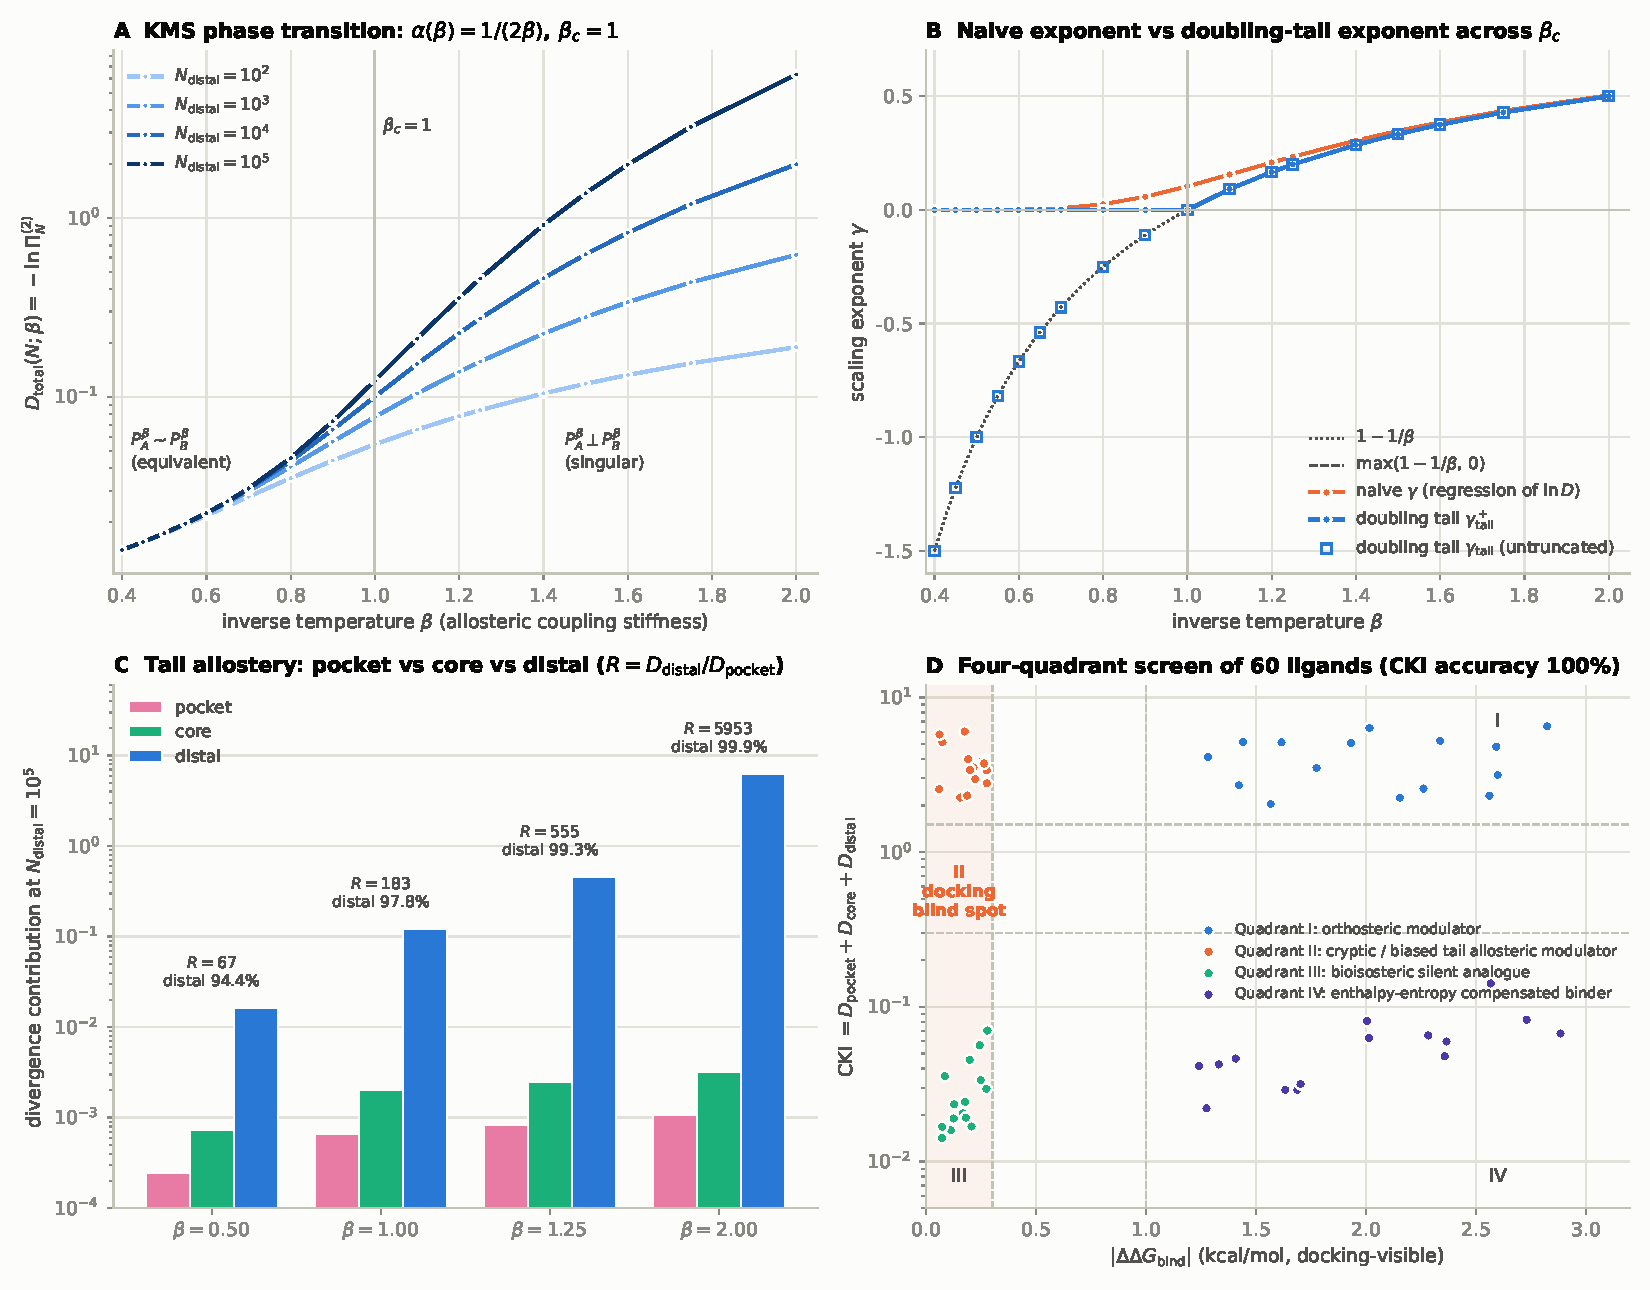
\includegraphics[width=\textwidth]{fig04_tail_allostery_kms_phase.pdf}
\caption{KMS temperature scaling and tail allostery (Theorem~\ref{thm:kms}, Corollary~\ref{cor:quadrant}; from \cite{ChenChen2026IV}). A: total index against $\beta$ for four system sizes; the curves separate at $\beta_c=1$. B: naive and doubling-tail exponents; the doubling exponent follows $\max(1-1/\beta,0)$. C: pocket, core and distal contributions at $N=10^5$. D: sixty model ligands in the plane of pocket affinity change and total index.}
\label{fig:kms}
\end{figure}

\subsection*{Broken phases and the chemical obstruction group}
A multi-subunit allosteric macromolecule has several macroscopic two-state degrees of freedom, as in the Monod--Wyman--Changeux picture \cite{MWC1965}. Let there be $K=3$ of them, with conformational symmetry group $G_{\mathrm{conf}}=(\Z/2\Z)^3$. Perturbations act through a semigroup $S=P_0\sqcup R_1\sqcup R_2\sqcup R_3$. The substituent operators of channel $R_n$ flip bit $n$ and have energy levels $N_{n,m}=\lceil m^{1/\beta_n}\rceil$, so that $|R_n\cap[1,X]|=\lfloor X^{\beta_n}\rfloor$; $P_0$ acts trivially. Occupation numbers are geometric, $\PP(v_p\ge k)=N_p^{-\beta k}$, and the conformational sign $u_n$ of bit $n$ is uniform under the symmetric state \cite{ChenChen2026V}.

\begin{theorem}[The chemical obstruction group \cite{ChenChen2026V}]\label{thm:xi}
Let $\Xib=\{\chi\in\widehat{G_{\mathrm{conf}}}:\sum_{p\in S}N_p^{-\beta}|1-\chi(g_p)|^2<\infty\}$ and $A_\beta=\{n:\beta>\beta_n\}$. Then:
\begin{enumerate}[label=\textup{(\arabic*)},leftmargin=*]
\item $\Xib\cong(\Z/2\Z)^{A_\beta}$; the extremal equilibrium phases number $2^{|A_\beta|}$, and the residual symmetry group has order $8/2^{|A_\beta|}$;
\item the partition function $\zeta_S(\beta)=\zeta(\beta)-1$ converges only for $\beta>\beta_c=1$, so every breaking threshold satisfies $\beta_n\le\beta_c$;
\item for $\beta>\beta_n$ the order parameter $\Psi_n=u_n(-1)^{\sum_{p\in R_n}v_p}$ is defined almost surely by the Borel--Cantelli lemma and is invariant under every finite word of the semigroup; for $\beta\le\beta_n$ it does not exist;
\item the condensed order parameters are independent fair signs, and the relative entropy of an extremal phase with respect to the symmetric state is $|A_\beta|\ln2$.
\end{enumerate}
\end{theorem}

With thresholds $\beta_3=0.40<\beta_2=0.60<\beta_1=0.80<\beta_c=1$ the group grows from $\{1\}$ to $(\Z/2\Z)^3$ in three steps. The relative entropy is a staircase with one jump of $\ln2$ at each threshold, reproduced by simulation to $3.3\times10^{-3}$ nat at $18$ temperatures, and to $1.5\times10^{-3}$ nat after the Miller--Madow correction. The finite-word invariance was tested in $4\times10^5$ trials without a failure, whereas the uncompensated sign fails at the predicted rates $0.41875$, $0.17975$ and $0.05000$ (Figure~\ref{fig:xi}).

The obstruction group is the algebraic counterpart of Proposition~\ref{prop:tilt}. An extremal phase is selected by a tail-measurable order parameter, which no finite perturbation can change. A ligand that selects a phase therefore does something no pocket-local energy can do, and the information it fixes, $\ln2$ per condensed bit, is invisible in any finite window.

\begin{figure}[t]
\centering
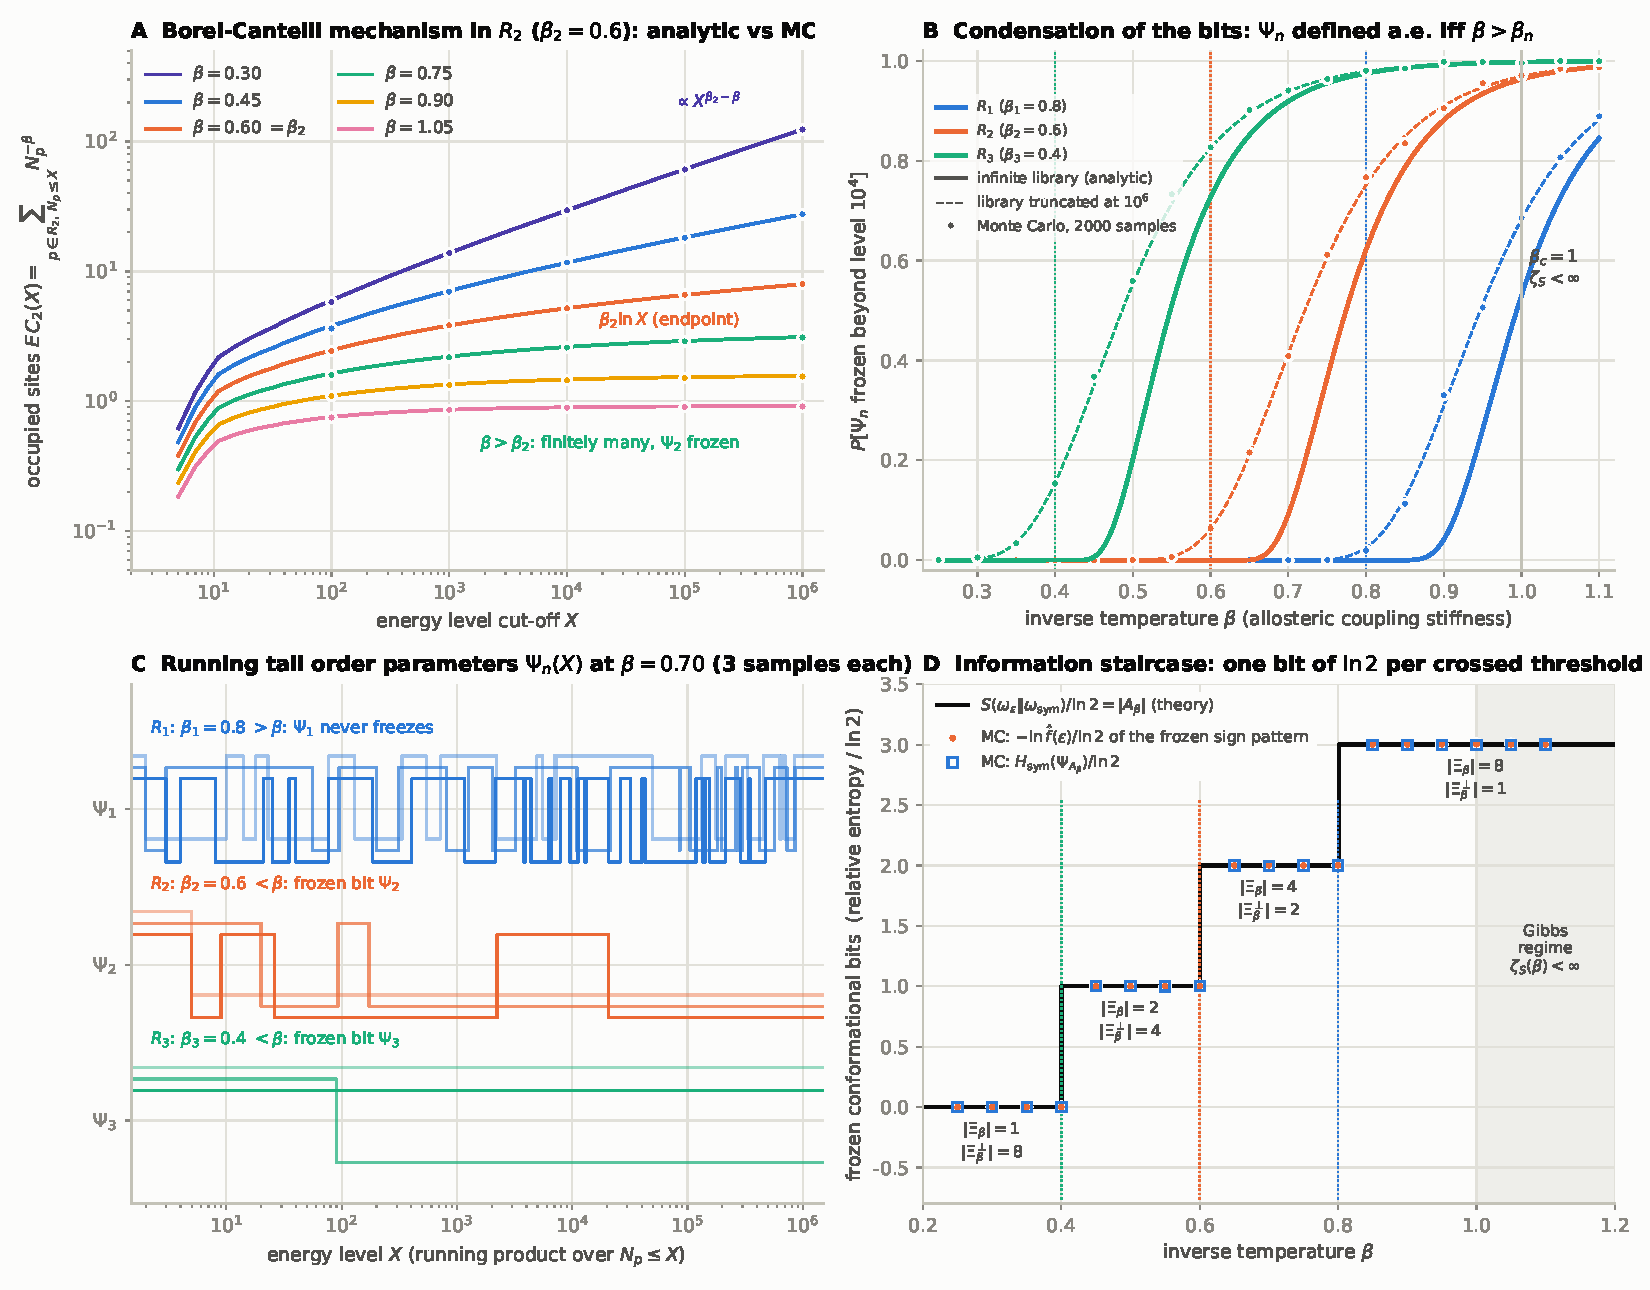
\includegraphics[width=\textwidth]{fig05_chemical_obstruction_group.pdf}
\caption{Broken phases and the obstruction group (Theorem~\ref{thm:xi}; from \cite{ChenChen2026V}). A: Borel--Cantelli growth of occupied sites in one channel. B: probability that an order parameter is frozen beyond a finite level, zero up to each threshold in the infinite system. C: running order parameters at $\beta=0.70$. D: relative-entropy staircase with the orders of the obstruction group and of the residual symmetry group.}
\label{fig:xi}
\end{figure}

%%%%%%%%%%%%%%%%%%%%%%%%%%%%%%%%%%%%%%%%%%%%%%%%%%%%%%%%%%%%%%%%%%%%%%%%%%%%%%%
\section{Cone-geodesic Wasserstein geometry and alchemical pathway topology}
\label{sec:wasserstein}

Mutual singularity says that two broken phases are distinguishable with certainty; it does not say how costly it is to move the ensemble from one to the other. The cost is a transport distance \cite{KantorovichRubinstein1958,Villani2009}, dual to a Lipschitz seminorm of the kind used for quantum metric spaces \cite{Connes1989,Rieffel1999}.

\subsection*{Wasserstein separation of broken phases}
Let a configuration be $x=(v,u)$ with occupation numbers $v\in\N_0^J$ and a macroscopic sign $u=\pm1$. The broken phases $\varphi_\pm$ have independent geometric occupations $\PP(v_j\ge k)=t_j^k$ and the sign locked to their parity, $u=\pm(-1)^{\sum_jv_j}$ \cite{ChenChen2026VI}. With $\Delta_0$ the sign flip, $\Delta_j$ the forward step of $v_j$ and weights $w_0,w_j$, the cone seminorm and the tail transport cost are
\begin{equation}\label{eq:wtail}
L(f)=\sup_x\Bigl(\frac{|\Delta_0f|^2}{w_0^2}+\sum_j\frac{|\Delta_jf|^2}{w_j^2}\Bigr)^{1/2},\qquad \Wtail=W_1(\varphi_+,\varphi_-)=\sup_{L(f)\le1}\bigl(\varphi_+(f)-\varphi_-(f)\bigr).
\end{equation}
The phases differ only through a tail-measurable sign, so $\Wtail$ is the minimal cost of the conversion that Theorem~\ref{thm:xi} forbids for finite perturbations.

\begin{theorem}[Bounds and exact values of the tail transport cost \cite{ChenChen2026VI}]\label{thm:wtail}
Let $m_j=(1-t_j)/(1+t_j)$, $\tau_j=1-m_j$ and $\Pi_\infty=\prod_jm_j$.
\begin{enumerate}[label=\textup{(\arabic*)},leftmargin=*]
\item $w_0\Pi_\infty\le\Wtail\le w_0$, and $\Pi_\infty>0$ if and only if $\sum_jt_j<\infty$ (Kakutani).
\item If $2\sum_jw_j^2t_j/(1-t_j)\le w_0^2$, the first-order odd Walsh chaos gives $\Wtail\ge\Pi_\infty\bigl(w_0^2+4\sum_jw_j^2t_j^2/(1-t_j)^2\bigr)^{1/2}$.
\item The relaxation in which every move changes one coordinate has the exact value $B_{\mathrm{scan}}=w_0\Pi_\infty+\sum_kw_{j_k}\tau_{j_k}\prod_{l<k}m_{j_l}$, with the weights truncated at $w_0$ and taken in ascending order. Consequently $\Wtail\le B_{\mathrm{scan}}$.
\end{enumerate}
\end{theorem}

On the benchmark $w_0=1$, $w=(\tfrac12,\tfrac13,\tfrac14)$, $t=(\tfrac12,\tfrac13,\tfrac15)$, the bounds are exact rationals: $1/9$ from item~(1), $35/216$ from item~(2), and $5/12$ from item~(3), which the five other scan orders exceed ($31/72$ to $37/72$). A log-barrier interior-point method on truncated lattices gives a strictly feasible primal point and a Lagrange dual certificate. Together with an explicit geometric tail bound they enclose the infinite-lattice value in
\[
\Wtail\in[0.229028,\ 0.229032].
\]
Truncated lattices give $0.22647$ and $0.22839$, inside the finite-lattice window $[0.2254,0.2288]$; the limit lies $2.3\times10^{-4}$ above it. The gap between $\Wtail$ and the scan barrier, $0.229$ against $0.417$, is the value of moving several coordinates at once.

\subsection*{Cone geodesics and cooperative moves}
On the residue lattice $\{0,1\}^k$ with forward differences, the cone seminorm defines a distance $d_L(\mathbf0,\mathbf1_k)$ between the unswitched and the fully switched state.

\begin{theorem}[Cone-geodesic recursion \cite{ChenChen2026VI}]\label{thm:cone}
$d_L(\mathbf0,\mathbf1_k)=h(\mathbf0)$, where $h(\mathbf1_k)=0$ and $h(x)$ is the largest root of $\sum_{j:x_j=0}((h-h(x+e_j))/w_j)^2=1$. For equal weights $d_L=w\sum_{m\le k}m^{-1/2}$; for two residues $d_L=w(1+1/\sqrt2)=1.707107\,w$, $14.64\%$ below two sequential flips. For all weights $\|w\|_2\le d_L\le\sum_jw_j$.
\end{theorem}

The recursion is the discrete eikonal equation of the $\infty$-Laplacian \cite{PSSW2009}, solved from the top of the lattice down. The $m$-th to last residue costs $w/\sqrt m$ because it moves together with $m-1$ others.

\subsection*{Alchemical paths}
The same geometry governs free-energy perturbation \cite{Zwanzig1954}. Let $k$ residues switch between two states under coupling parameters $\lambda_j$, with populations $p_j(\lambda_j)$. The Fisher metric of the family is flat in the coordinates $\theta_j=2\arcsin\sqrt{p_j}$, so the thermodynamic length \cite{Crooks2007,SivakCrooks2012} of a path switching the residues one at a time is $\sum_jL_j$, while the cooperative geodesic has length $\|L\|_2$. Define the path group $\Xi(P)$ as the subgroup of $(\Z/2\Z)^k$ generated by the sets of residues switched together in single steps.

\begin{proposition}[Path topology and sampling cost \cite{ChenChen2026VI}]\label{prop:fep}
All paths share $\Delta G$. At equal total sampling, the variance of the exponential-averaging estimator along a path equally spaced in thermodynamic length is $\mathcal L(P)^2/(nM)$ to leading order, so the variance ratio of the sequential and cooperative paths tends to $(\sum_jL_j/\|L\|_2)^2$. The sequential path has $\Xi(P)=(\Z/2\Z)^k$; the cooperative path has $\Xi(P)=\{0,e_1+\dots+e_k\}$.
\end{proposition}

For three residues with lengths $(2,\tfrac43,1)$ and $\Delta G=-4.941581\,k_BT$ on every path, the lengths are $4.3333$ and $2.6034$. The predicted variance ratio is $2.77$, measured as $2.72$ to $3.19$ over six window counts, so the cooperative schedule needs about $64\%$ fewer samples. The model has independent residues and exact sampling; the result has not been tested in molecular dynamics (Section~\ref{sec:discussion}). Figure~\ref{fig:wasserstein} summarises the section.

\begin{figure}[t]
\centering
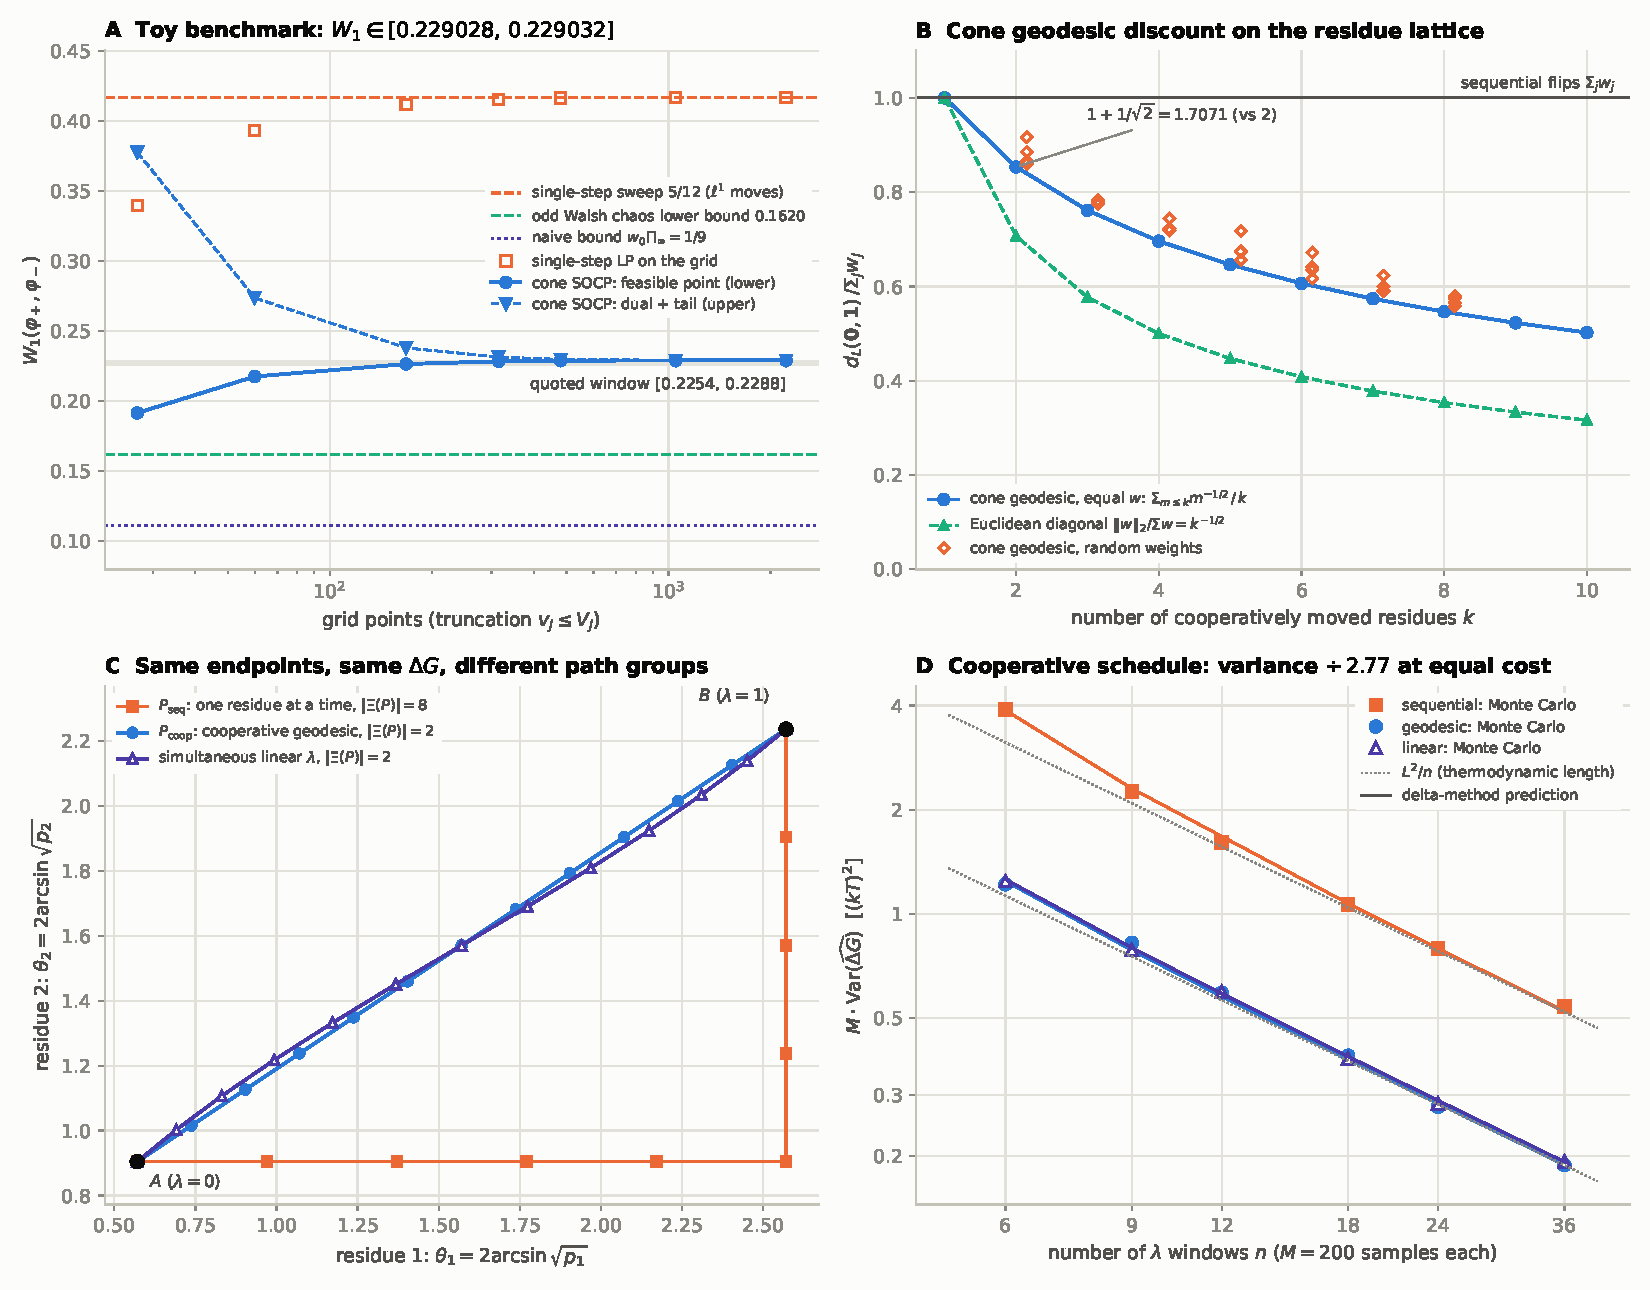
\includegraphics[width=\textwidth]{fig06_cone_geodesic_wasserstein.pdf}
\caption{Transport cost between broken phases and cooperative moves (Theorems~\ref{thm:wtail}, \ref{thm:cone}, Proposition~\ref{prop:fep}; from \cite{ChenChen2026VI}). A: lower and upper bounds for $\Wtail$ against lattice size, with the scan barrier $5/12$ and the Walsh and squeeze bounds. B: cone-geodesic distance relative to sequential flips. C: three alchemical paths with the same endpoints in flat Fisher coordinates. D: variance of the free-energy estimate against the number of windows.}
\label{fig:wasserstein}
\end{figure}

%%%%%%%%%%%%%%%%%%%%%%%%%%%%%%%%%%%%%%%%%%%%%%%%%%%%%%%%%%%%%%%%%%%%%%%%%%%%%%%
\section{Algorithmic pipeline for molecular-dynamics trajectories and tail-augmented representations}
\label{sec:pipeline}

\subsection*{From ensembles to trajectories}
The theorems above concern exact ensembles. A molecular-dynamics trajectory supplies $T$ correlated frames of $D=3N_{\mathrm{res}}$ coordinates, and three obstacles stand between it and the indices \cite{ChenChen2026VII}. Rigid-body motion must be removed jointly for the two ensembles compared. The sample covariance is singular: after superposition it has six null directions, and for $T\le D$ its rank is at most $T-1$, so the index is infinite. Finally, even a regularised index of two samples of the same ensemble is far from zero. The open Python package \texttt{kakutani\_pharma} implements the following remedies.

\begin{enumerate}[label=(\arabic*),leftmargin=*]
\item \emph{Joint superposition and rigidity.} All frames of both ensembles are superimposed on their common mean by iterated mass-weighted Kabsch rotations \cite{Kabsch1976}. For elastic-network models, $\dim\ker H=6$ holds if and only if the network is infinitesimally rigid \cite{AsimowRoth1978}. Two rigid halves joined by $c<6$ independent springs have $12-c$ zero modes, which explained the $11$ zero modes of a first benchmark geometry.
\item \emph{Shrinkage.} The analytical Ledoit--Wolf estimator \cite{LedoitWolf2004} is positive definite for any number of frames and keeps the three-way decomposition of Theorem~\ref{thm:decomp}. With $200$ frames in $360$ dimensions the sample index is infinite and the shrunk one is $66.18$.
\item \emph{Split-trajectory null.} The excess $\DCKI=\frac12[\CKI(A_1,B_1)+\CKI(A_2,B_2)]-\frac12[\CKI(A_1,A_2)+\CKI(B_1,B_2)]$ over contiguous halves is unbiased under the null up to $O(\tau/h)$. An independent replica falls from a raw index of $3.10$ to $0.010\,[-0.101,0.118]$.
\item \emph{Within-half block bootstrap.} Blocks must be resampled inside each half \cite{Kunsch1989}. Resampling before splitting leaks about $40\%$ of the blocks across halves and inflates the excess by about $3.0$. The residual duplicate-frame bias ($+0.126$ for a local ligand) is reported with bias-shifted and basic intervals \cite{EfronTibshirani1993}.
\item \emph{Shell scaling.} The excess over pocket-centred shells $S(r)$ gives a curve whose population version is nondecreasing and exactly flat beyond a pocket-local perturbation, also in the rigid-body gauge; this is the mechanism of Proposition~\ref{prop:tilt}. The distal exponent $\gamma$ is its log-log slope.
\end{enumerate}

On a synthetic four-domain benchmark with a local substrate, a distal effector and an independent replica, the sample exponents are $\gamma=0.12\,[0.05,0.30]$, $1.36\,[1.30,1.46]$ and $0.88\,[0.80,0.91]$ for the substrate, the effector and both. The exact population values are $0$, $1.34$ and $0.90$. The replica's excess is consistent with zero at every shell, and the first-order index places $9/10$, $10/10$ and $10/10$ of its top residues in the perturbed sets (Figure~\ref{fig:pipeline}).

\begin{figure}[t]
\centering
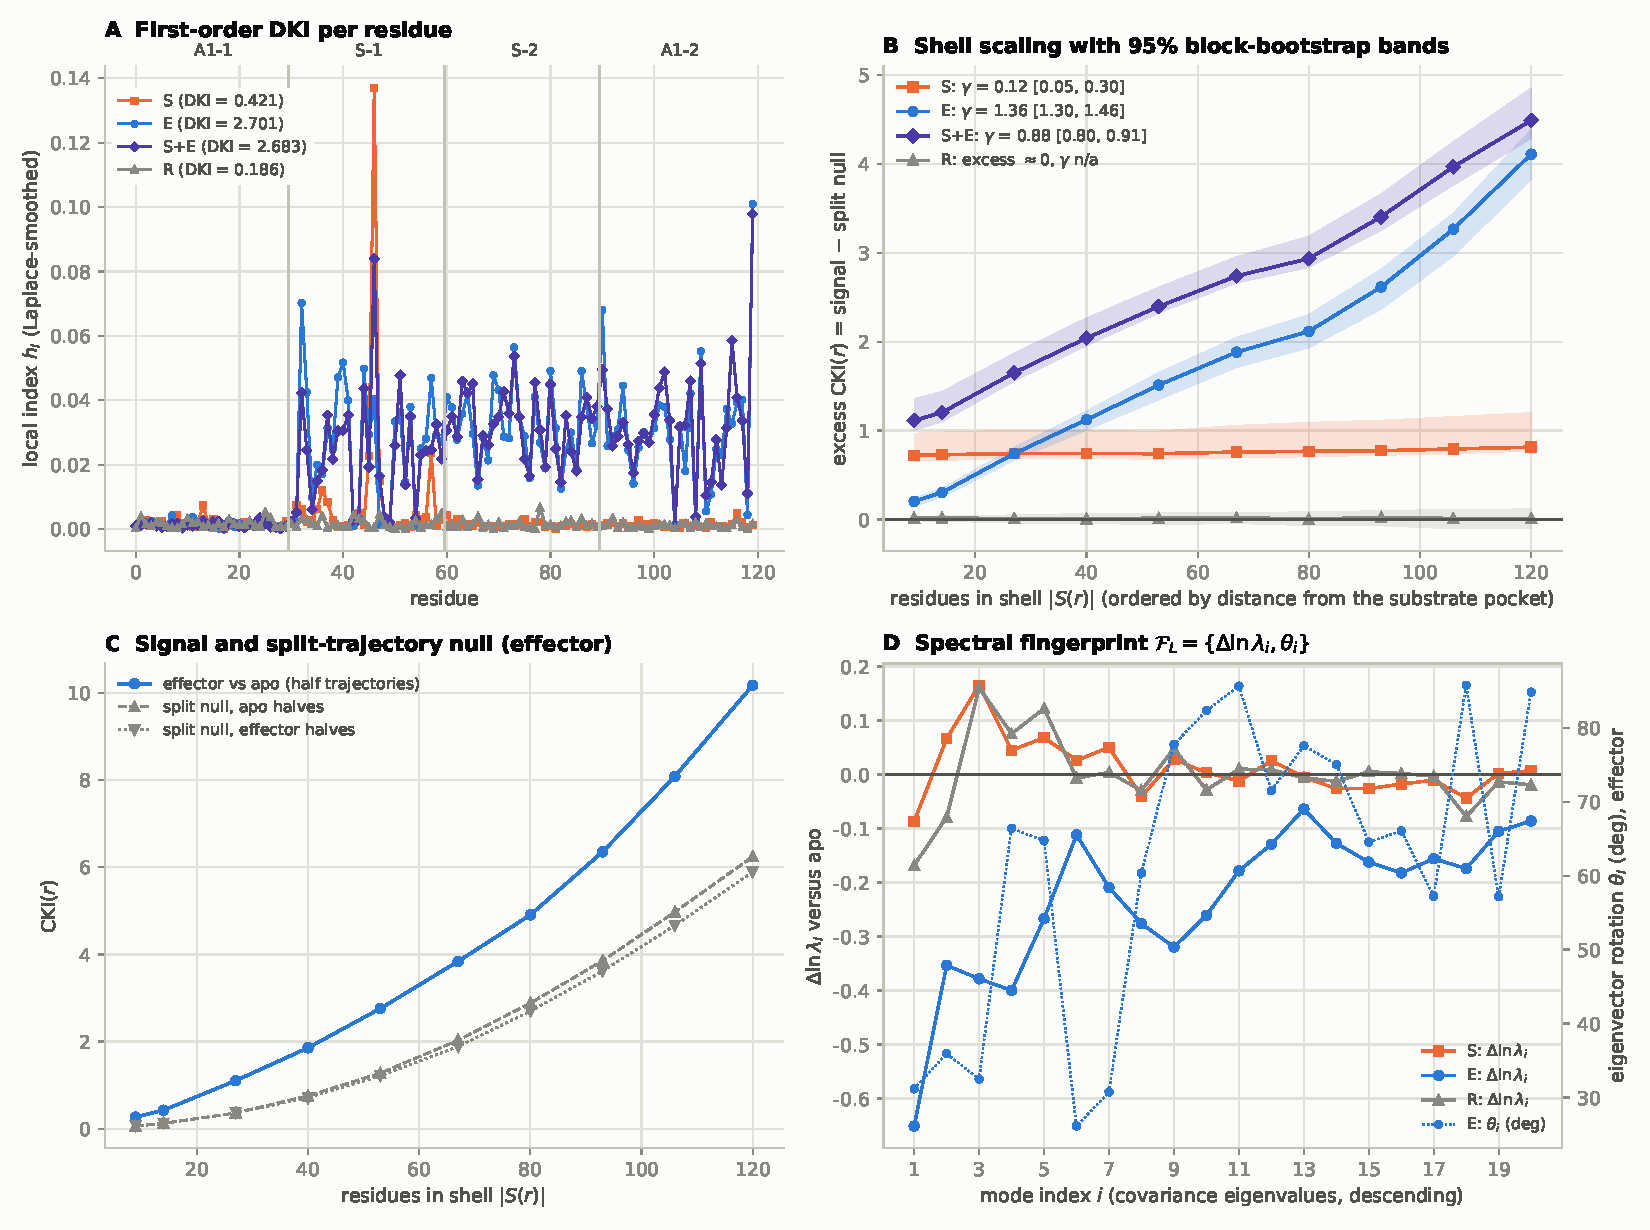
\includegraphics[width=\textwidth]{fig07_kakutani_diagnostics.pdf}
\caption{Diagnostics of the estimation pipeline on a synthetic four-domain protein (from \cite{ChenChen2026VII}). A: first-order index per residue. B: null-corrected excess over pocket-centred shells with within-half bootstrap bands; the local substrate is flat beyond the pocket and the distal effector grows through the protein. C: signal and split-trajectory null. D: spectral fingerprint.}
\label{fig:pipeline}
\end{figure}

\subsection*{Tail-augmented molecular representations}
Descriptors of protein--ligand complexes used for scoring and learning are overwhelmingly local: features of the pocket, the pose and the interaction. By Theorem~\ref{thm:blind} no function of such features can resolve the measure class of the global ensemble. We therefore propose to append two blocks, one for each kind of information the theory identifies.

\begin{definition}[Tail-augmented representation]\label{def:rep}
For a ligand $L$ with a reference ensemble, let $z(L)=z_{\mathrm{local}}\oplus z_{\mathrm{symmetry}}\oplus z_{\mathrm{tail}}$ with
\begin{enumerate}[label=\textup{(\roman*)},leftmargin=*]
\item $z_{\mathrm{local}}$: pocket descriptors, such as the pocket affinity change, the pocket RMSD, the first-order index of the pocket residues and the pocket-shell excess $\DCKI(r_0)$;
\item $z_{\mathrm{symmetry}}$: the phase label, namely the set $A_\beta$ of condensed conformational bits, their frozen order parameters $\Psi_n$, and the orders of $\Xib$ and of the residual symmetry group, estimated from the frozen fractions of the order parameters \cite{ChenChen2026V};
\item $z_{\mathrm{tail}}$: the null-corrected excess over all residues, the distal exponent $\gamma$ or the doubling-tail exponent, the rotation share $D_{\mathrm{rot}}/D_{\mathrm{cov}}$, and the fingerprint entries $(\Delta\ln\lambda_i,\theta_i)$ that exceed the replica scatter.
\end{enumerate}
\end{definition}

\begin{proposition}[What the added blocks carry]\label{prop:rep}
\begin{enumerate}[label=\textup{(\arabic*)},leftmargin=*]
\item There are ligand pairs with identical $z_{\mathrm{local}}$, and identical per-residue features, whose ensembles are mutually singular and whose $z_{\mathrm{tail}}$ differ; no classifier based on $z_{\mathrm{local}}$ separates them.
\item For ligands acting by pocket-local energies, the population value of the distal exponent in $z_{\mathrm{tail}}$ is zero, and the excess over all residues equals its value at the pocket shell. The tail block therefore does not duplicate the pocket block.
\item On the four-quadrant benchmark of Corollary~\ref{cor:quadrant}, a pocket-only call is correct for $30$ of $60$ ligands and recognises none of the tail-allosteric class, while the call using the pocket affinity together with the total index is correct for all $60$.
\end{enumerate}
\end{proposition}

\begin{proof}
(1) is Theorem~\ref{thm:blind} with the finite-size growth of Theorems~\ref{thm:trichotomy} and~\ref{thm:dominance}. (2) is Proposition~\ref{prop:tilt} applied to every shell containing the pocket: the Bhattacharyya coefficient equals that of the pocket marginal, so the curve is constant and its slope vanishes. (3) is Corollary~\ref{cor:quadrant}.
\end{proof}

The proposition is a statement about information, not about learning performance. Whether the added blocks improve a trained predictor of efficacy or selectivity on real data has not been tested. The blocks require simulation of each complex, and $z_{\mathrm{symmetry}}$ applies only where the conformational degrees of freedom have the multi-bit structure of Section~\ref{sec:kms}.

%%%%%%%%%%%%%%%%%%%%%%%%%%%%%%%%%%%%%%%%%%%%%%%%%%%%%%%%%%%%%%%%%%%%%%%%%%%%%%%
\section{Discussion: what is established, what is not, and what follows}
\label{sec:discussion}

\subsection*{Established}
The blindness theorem and the proposition on pocket-local tilts (Section~\ref{sec:intro}) are proved here in full. The theorems of Sections~\ref{sec:dki}--\ref{sec:pipeline} are proved in Papers I--VII, with complete proofs and with every quoted constant reproduced by scripts that are archived with each paper. Among them are the critical exponent $\alpha_c=\tfrac12$ and the universal doubling increment; the three-way decomposition with $D_{\mathrm{rot}}\ge0$; the Szeg\H{o} rate of covariance dominance; the joint spectral phase diagram; the KMS trichotomy and the tail-allostery amplification; the structure of the obstruction group and the relative-entropy staircase; and the bounds, exact values and enclosure of $\Wtail$. The same holds for the cone-geodesic recursion, the zero-mode count, the positivity of the shrinkage, the null subtraction and the exact plateau of local perturbations.

\subsection*{Not established}
\begin{sloppypar}
\emph{Models versus molecules.} Every number in this article comes from analytic models (product measures, Gaussian and Toeplitz ensembles, elastic networks, multi-bit switch systems) or from synthetic trajectories with known ground truth. None comes from an all-atom simulation or an experiment on a real protein--ligand system. The theory states what a local description \emph{can} miss and how to measure it. Whether a given ligand pair of pharmacological interest lies in the singular or the equivalent regime is an empirical question.
\emph{Idealisation.} The dichotomies are statements about infinite systems. A protein is finite, and every finite-dimensional affinity is positive. The finite-size theory (Theorems~\ref{thm:trichotomy}, \ref{thm:fss}, \ref{thm:spectral} and~\ref{thm:kms}) is what connects the two: in the singular regime the index grows as a power of the system size, and the doubling increment reads the exponent without the bias of the Euler--Maclaurin constant.
\emph{Gaussian and harmonic approximations.} The correlated index is the Bhattacharyya distance of Gaussian approximations. Multimodal ensembles with several metastable basins are only partly described by it, and the first-order index on discrete states covers part of the remainder.
\emph{Parameters of the mechanisms.} The inverse temperature $\beta$ of Section~\ref{sec:kms} and the channel exponents of the obstruction group are model parameters. Their identification with measurable stiffnesses or with the density of states of specific residue networks has not been made.
\emph{Representation.} The tail-augmented representation is a proposal whose information content is established (Proposition~\ref{prop:rep}), but whose value for predictive models is untested.
\emph{Transport cost.} The enclosure of $\Wtail$ is computer-assisted in double precision without interval arithmetic, and the Walsh bound requires the feasibility condition of Theorem~\ref{thm:wtail}(2). The sampling advantage of cooperative alchemical paths is established for independent residues with exact sampling only.
\end{sloppypar}

\subsection*{Relation to the literature}
The dichotomies are Kakutani's \cite{Kakutani1948} and Feldman--H\'ajek's \cite{Feldman1958,Hajek1958}. The thermodynamic language is that of KMS states \cite{HHW1967,BratteliRobinson1997} and of the Bost--Connes system \cite{BostConnes1995} in its localized form \cite{Chen2026}. The pharmacological premises, namely the ensemble nature of allostery, cryptic sites and concerted transitions, are those of \cite{Motlagh2014,Bowman2012,MWC1965}. Elastic network models \cite{Tirion1996,Atilgan2001} supply the harmonic benchmark. Transport distances and quantum metrics come from \cite{KantorovichRubinstein1958,Villani2009,Connes1989,Rieffel1999}. Thermodynamic length and free-energy estimation come from \cite{Crooks2007,SivakCrooks2012,Zwanzig1954,ShirtsChodera2008}. Covariance shrinkage and resampling for dependent data come from \cite{LedoitWolf2004,Kunsch1989,EfronTibshirani1993}. What is new is the combination: a measure-class criterion for the global effect of a ligand, the identification of its critical exponents and invariants across first-order, correlated, spectral, thermal, algebraic and transport descriptions, and an estimation pipeline that turns it into numbers with controlled bias.

\subsection*{Outlook}
The immediate test is empirical. Unliganded and liganded all-atom trajectories of a multi-domain allosteric enzyme, with independent replicas, should show a replica excess consistent with zero, and a distal exponent that separates ligands acting in the pocket from ligands acting through the interfaces. A second test is comparative: pairs of ligands with similar affinity and different functional outcomes should differ in $z_{\mathrm{tail}}$ and not in $z_{\mathrm{local}}$. A third concerns alchemical practice: the ordering of coupling parameters in multi-residue transformations can be chosen by thermodynamic length, and the predicted variance ratios can be checked against simulation. On the theoretical side, the extension beyond Gaussian ensembles to mixtures over metastable basins, and the identification of the channel exponents from structural data, are the main open problems.

\subsection*{Data availability}
{\raggedright
This article is archived under DOI \href{https://doi.org/10.5281/zenodo.23042828}{10.5281/zenodo.23042828} and maintained at \url{https://github.com/Ruqing1963/kakutani-statistical-pharmacology-synthesis}. The checks made for it are in \texttt{code/verify\_synthesis\_theorems.py}, which writes \texttt{results/synthesis\_verification.txt}. They cover the expansion \eqref{eq:htaylor} to eighth order, the pair divergence of Theorem~\ref{thm:blind}(2) and its partial sums, Proposition~\ref{prop:tilt} on a Gaussian example, and the constants of Theorem~\ref{thm:dominance}. All other code, data, figures and derived tables are archived with the individual papers: Paper~I, DOI 10.5281/zenodo.23005921 (version 1.1: 10.5281/zenodo.23018827); Paper~II, 10.5281/zenodo.23012217; Paper~III, 10.5281/zenodo.23015709 (version 1.1: 10.5281/zenodo.23019056); Paper~IV, 10.5281/zenodo.23018236; Paper~V, 10.5281/zenodo.23027704; Paper~VI, 10.5281/zenodo.23029360; Paper~VII, including the \texttt{kakutani\_pharma} package, 10.5281/zenodo.23039869. The monograph is DOI 10.5281/zenodo.22883179.
\par}

\subsection*{Funding}
This project was supported by the National Natural Science Foundation of China (No.~22464010), the Guangxi Natural Science Foundation of China (No.~2025GXNSFAA069294), and the 2025 Bagui Youth Top Talent Project.

\begin{thebibliography}{99}
\bibitem{AsimowRoth1978} L.~Asimow and B.~Roth, \emph{The rigidity of graphs}, Trans. Amer. Math. Soc. \textbf{245} (1978), 279--289.
\bibitem{Atilgan2001} A.~R. Atilgan, S.~R. Durell, R.~L. Jernigan, M.~C. Demirel, O.~Keskin and I.~Bahar, \emph{Anisotropy of fluctuation dynamics of proteins with an elastic network model}, Biophys. J. \textbf{80} (2001), 505--515.
\bibitem{Bhattacharyya1943} A.~Bhattacharyya, \emph{On a measure of divergence between two statistical populations defined by their probability distributions}, Bull. Calcutta Math. Soc. \textbf{35} (1943), 99--109.
\bibitem{BostConnes1995} J.-B. Bost and A.~Connes, \emph{Hecke algebras, type III factors and phase transitions with spontaneous symmetry breaking in number theory}, Selecta Math. (N.S.) \textbf{1} (1995), 411--457.
\bibitem{Bowman2012} G.~R. Bowman and P.~L. Geissler, \emph{Equilibrium fluctuations of a single folded protein reveal a multitude of potential cryptic allosteric sites}, Proc. Natl. Acad. Sci. USA \textbf{109} (2012), 11681--11686.
\bibitem{BratteliRobinson1997} O.~Bratteli and D.~W. Robinson, \emph{Operator Algebras and Quantum Statistical Mechanics 2}, 2nd ed., Springer, Berlin, 1997.
\bibitem{Chen2026} R.~Chen, \emph{Localized Bost--Connes systems}, assembled from the thirty-nine papers of the series, 2026, DOI 10.5281/zenodo.22883179.
\bibitem{ChenChen2026I} Z.~Chen and R.~Chen, \emph{Statistical pharmacology via Kakutani dichotomy I: the marginal drug Kakutani index and the $\alpha_c=1/2$ criticality theorem in high-dimensional conformational ensembles}, 2026, DOI 10.5281/zenodo.23005921 (version 1.1: 10.5281/zenodo.23018827).
\bibitem{ChenChen2026II} Z.~Chen and R.~Chen, \emph{Statistical pharmacology via Kakutani dichotomy II: the correlated Kakutani index, the 99.95\% covariance dominance theorem, and spectral fingerprints of cryptic allostery}, 2026, DOI 10.5281/zenodo.23012217.
\bibitem{ChenChen2026III} Z.~Chen and R.~Chen, \emph{Statistical pharmacology via Kakutani dichotomy III: spectral Kakutani--Feldman--H\'ajek criticality of correlated conformational modes: mode amplitude perturbation, iso-spectral Givens rotation, and tail-increment finite-size elimination}, 2026, DOI 10.5281/zenodo.23015709 (version 1.1: 10.5281/zenodo.23019056).
\bibitem{ChenChen2026IV} Z.~Chen and R.~Chen, \emph{Statistical pharmacology via Kakutani dichotomy IV: KMS inverse-temperature criticality $\beta_c=1$, pocket-to-distal tail allostery, and the four-quadrant ligand classification}, 2026, DOI 10.5281/zenodo.23018236.
\bibitem{ChenChen2026V} Z.~Chen and R.~Chen, \emph{Statistical pharmacology via Kakutani dichotomy V: the chemical obstruction group $\Xi_\beta^{\mathrm{drug}}(S)$, Borel--Cantelli tail order parameters, and the relative-entropy staircase}, 2026, DOI 10.5281/zenodo.23027704.
\bibitem{ChenChen2026VI} Z.~Chen and R.~Chen, \emph{Statistical pharmacology via Kakutani dichotomy VI: Wasserstein phase separation $W_1(\varphi_+,\varphi_-)$, the single-step scan barrier, and cone-geodesic collective moves}, 2026, DOI 10.5281/zenodo.23029360.
\bibitem{ChenChen2026VII} Z.~Chen and R.~Chen, \emph{Statistical pharmacology via Kakutani dichotomy VII: the kakutani\_pharma pipeline, Ledoit--Wolf regularized CKI, split-trajectory null subtraction, and shell-scaling exponents in multi-domain allostery}, 2026, DOI 10.5281/zenodo.23039869.
\bibitem{Connes1989} A.~Connes, \emph{Compact metric spaces, Fredholm modules, and hyperfiniteness}, Ergodic Theory Dynam. Systems \textbf{9} (1989), 207--220.
\bibitem{Crooks2007} G.~E. Crooks, \emph{Measuring thermodynamic length}, Phys. Rev. Lett. \textbf{99} (2007), 100602.
\bibitem{EfronTibshirani1993} B.~Efron and R.~J. Tibshirani, \emph{An Introduction to the Bootstrap}, Chapman \& Hall, New York, 1993.
\bibitem{Feldman1958} J.~Feldman, \emph{Equivalence and perpendicularity of Gaussian processes}, Pacific J. Math. \textbf{8} (1958), 699--708.
\bibitem{Fiedler1971} M.~Fiedler, \emph{Bounds for the determinant of the sum of Hermitian matrices}, Proc. Amer. Math. Soc. \textbf{30} (1971), 27--31.
\bibitem{GrenanderSzego1958} U.~Grenander and G.~Szeg\H{o}, \emph{Toeplitz Forms and Their Applications}, University of California Press, Berkeley, 1958.
\bibitem{HHW1967} R.~Haag, N.~M. Hugenholtz and M.~Winnink, \emph{On the equilibrium states in quantum statistical mechanics}, Comm. Math. Phys. \textbf{5} (1967), 215--236.
\bibitem{Hajek1958} J.~H\'ajek, \emph{On a property of normal distributions of any stochastic process}, Czechoslovak Math. J. \textbf{8} (1958), 610--618.
\bibitem{Kabsch1976} W.~Kabsch, \emph{A solution for the best rotation to relate two sets of vectors}, Acta Cryst. A \textbf{32} (1976), 922--923.
\bibitem{Kakutani1948} S.~Kakutani, \emph{On equivalence of infinite product measures}, Ann. of Math. (2) \textbf{49} (1948), 214--224.
\bibitem{KantorovichRubinstein1958} L.~V. Kantorovich and G.~S. Rubinstein, \emph{On a space of completely additive functions}, Vestnik Leningrad. Univ. \textbf{13} (1958), no.~7, 52--59.
\bibitem{Kunsch1989} H.~R. K\"unsch, \emph{The jackknife and the bootstrap for general stationary observations}, Ann. Statist. \textbf{17} (1989), 1217--1241.
\bibitem{LedoitWolf2004} O.~Ledoit and M.~Wolf, \emph{A well-conditioned estimator for large-dimensional covariance matrices}, J. Multivariate Anal. \textbf{88} (2004), 365--411.
\bibitem{Motlagh2014} H.~N. Motlagh, J.~O. Wrabl, J.~Li and V.~J. Hilser, \emph{The ensemble nature of allostery}, Nature \textbf{508} (2014), 331--339.
\bibitem{MWC1965} J.~Monod, J.~Wyman and J.-P. Changeux, \emph{On the nature of allosteric transitions: a plausible model}, J. Mol. Biol. \textbf{12} (1965), 88--118.
\bibitem{PSSW2009} Y.~Peres, O.~Schramm, S.~Sheffield and D.~B. Wilson, \emph{Tug-of-war and the infinity Laplacian}, J. Amer. Math. Soc. \textbf{22} (2009), 167--210.
\bibitem{Rieffel1999} M.~A. Rieffel, \emph{Metrics on state spaces}, Doc. Math. \textbf{4} (1999), 559--600.
\bibitem{ShirtsChodera2008} M.~R. Shirts and J.~D. Chodera, \emph{Statistically optimal analysis of samples from multiple equilibrium states}, J. Chem. Phys. \textbf{129} (2008), 124105.
\bibitem{SivakCrooks2012} D.~A. Sivak and G.~E. Crooks, \emph{Thermodynamic metrics and optimal paths}, Phys. Rev. Lett. \textbf{108} (2012), 190602.
\bibitem{Tirion1996} M.~M. Tirion, \emph{Large amplitude elastic motions in proteins from a single-parameter, atomic analysis}, Phys. Rev. Lett. \textbf{77} (1996), 1905--1908.
\bibitem{Villani2009} C.~Villani, \emph{Optimal Transport: Old and New}, Springer, Berlin, 2009.
\bibitem{Zwanzig1954} R.~W. Zwanzig, \emph{High-temperature equation of state by a perturbation method. I. Nonpolar gases}, J. Chem. Phys. \textbf{22} (1954), 1420--1426.
\end{thebibliography}

\end{document}
